\chapter{Efficient Simulation} \label{julia-sim-chapter}

In some cases, we would like to optimize our simulations of nanowires more efficiently and in a 
more stable manner than in LTspice. In devices with hundreds of thousands of nanowires, LTspice
model optimizations can only go so far. This raises the need for a nanowire-centric simulation
environment. We designed a nanowire simulator in Julia, optimized for efficiently simulating 2-port 
nonlinear transmission lines. Since we care about time domain (TD) simulation for the types of nonlinearities
we exploit, the model was designed to simulate the time behavior of nanowires in a manner
similar to the phenomenological nanowire model \cite{phen_model}. We however also use
nonlinear frequency domain (FD) methods to simulate FD macro-models on the fly that are reused in the
TD simulation.


\section{Transmission Line Model}

We choose to model nanowires as nonlinear transmission lines encoding both nonlinearities
by default into the model. Using this method, we can get all the microwave characteristics of
the device by default and optimize for this topology. Unlike in LTspice where we had to optimize
the choice of nanowire model based on the microwave topology to increase performance, we design
a simulator around the nanowire nonlinear transmission line and as such guarantee optimizations
for the nanowire devices. On top of that, all devices on the same chip are superconducting, and
as such, a nanowire simulation environment can accurately model devices that are typically 
modeled only in the linear regime while preserving the optimizations granted by the nonlinear
solver.

The transmission line model is modeled similarly to the SNSPI presented in figure 
\ref{fig:snspi_tline}. Modeling all nanowire transmission lines (and SNSPDs) in an architecture similar to
the SNSPI is an accurate depiction of the true dynamics. Nanowire transmission lines exhibit the same
nonlinearities but can have a different photon behavior which can be encoded by the user. For example,
accounting for polarization, absorptive layers, etc. can be added on top of an efficient transmission line
model.

In the discrete sense that we care about for efficiently simulating for meanders with varying widths,
we can realize that any 2-terminal nanowire can simulate the same classes of devices with some added
differential equations. The basic nanowire model in the Julia simulator can model transmission lines,
SNSPDs, SNSPIs and even tapers with low overhead for complex geometries. It can be extended to work on 
n-terminal devices by coupling node voltages.

We chose to employ a hybrid fixed-variable time step method over SPICE's adaptive time step. WRspice uses a 
similar fixed time step simulator for simulating superconducting electronics \cite{wrspice}. 
\textbf{TODO TODO TODO TODO TODO TODO TODO TODO TODO TODO TODO TODO TODO TODO TODO TODO TODO TODO}

\subsection{Equivalent Circuit}

\begin{figure}
  \centering
  \subfigure[]{

\tikzset{every picture/.style={line width=0.75pt}} %set default line width to 0.75pt        

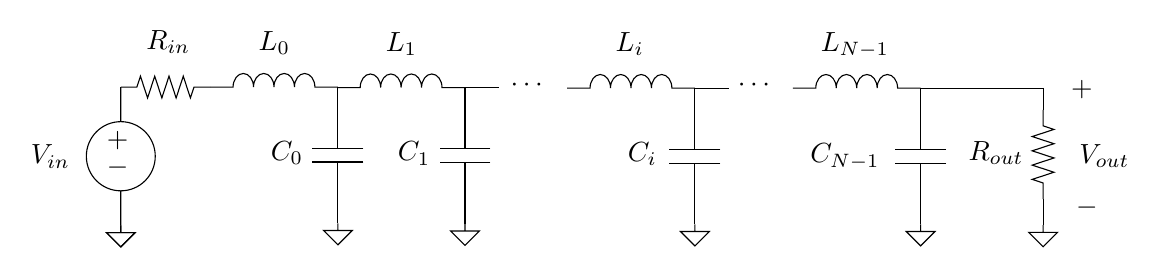
\begin{tikzpicture}[x=0.75pt,y=0.75pt,yscale=-1,xscale=1]
%uncomment if require: \path (0,170); %set diagram left start at 0, and has height of 170

%Shape: Capacitor [id:dp48936363235816716] 
\draw   (186.6,60.75) -- (186.6,90.29) (198.85,96.86) -- (174.35,96.86) (198.85,90.29) -- (174.35,90.29) (186.6,96.86) -- (186.6,126.4) ;
%Shape: Inductor (Air Core) [id:dp34831852124024465] 
\draw   (125,60.75) -- (136.09,60.75) .. controls (136.09,57.13) and (138.3,54.2) .. (141.02,54.2) .. controls (143.74,54.2) and (145.94,57.13) .. (145.94,60.75) .. controls (145.94,57.13) and (148.15,54.2) .. (150.87,54.2) .. controls (153.59,54.2) and (155.8,57.13) .. (155.8,60.75) .. controls (155.8,57.13) and (158.01,54.2) .. (160.73,54.2) .. controls (163.45,54.2) and (165.66,57.13) .. (165.66,60.75) .. controls (165.66,57.13) and (167.86,54.2) .. (170.58,54.2) .. controls (173.3,54.2) and (175.51,57.13) .. (175.51,60.75) -- (186.6,60.75) ;
%Shape: Output [id:dp10584432339741157] 
\draw   (82,77.41) .. controls (91.17,77.41) and (98.6,84.87) .. (98.6,94.08) .. controls (98.6,103.28) and (91.17,110.74) .. (82,110.74) .. controls (72.83,110.74) and (65.4,103.28) .. (65.4,94.08) .. controls (65.4,84.87) and (72.83,77.41) .. (82,77.41) -- cycle (82,60.75) -- (82,77.41) (82,127.4) -- (82,110.74) ;
%Shape: Ground [id:dp7430900812234964] 
\draw   (88.91,130.86) -- (82,137.77) -- (75.09,130.86) -- (88.91,130.86) -- cycle (82,127.4) -- (82,130.86) ;
%Shape: Resistor [id:dp42422759169539104] 
\draw   (82,60.75) -- (89.74,60.75) -- (91.46,55.5) -- (94.9,66) -- (98.34,55.5) -- (101.78,66) -- (105.22,55.5) -- (108.66,66) -- (112.1,55.5) -- (115.54,66) -- (117.26,60.75) -- (125,60.75) ;
%Shape: Ground [id:dp9822064397482662] 
\draw   (88.91,130.86) -- (82,137.77) -- (75.09,130.86) -- (88.91,130.86) -- cycle (82,127.4) -- (82,130.86) ;
%Shape: Ground [id:dp9718308390067569] 
\draw   (193.51,129.86) -- (186.6,136.77) -- (179.69,129.86) -- (193.51,129.86) -- cycle (186.6,126.4) -- (186.6,129.86) ;
%Shape: Capacitor [id:dp40912991408934096] 
\draw   (247.85,61) -- (247.85,90.54) (260.1,97.11) -- (235.6,97.11) (260.1,90.54) -- (235.6,90.54) (247.85,97.11) -- (247.85,126.65) ;
%Shape: Inductor (Air Core) [id:dp1706441962845362] 
\draw   (186.25,61) -- (197.34,61) .. controls (197.34,57.38) and (199.55,54.45) .. (202.27,54.45) .. controls (204.99,54.45) and (207.19,57.38) .. (207.19,61) .. controls (207.19,57.38) and (209.4,54.45) .. (212.12,54.45) .. controls (214.84,54.45) and (217.05,57.38) .. (217.05,61) .. controls (217.05,57.38) and (219.26,54.45) .. (221.98,54.45) .. controls (224.7,54.45) and (226.91,57.38) .. (226.91,61) .. controls (226.91,57.38) and (229.11,54.45) .. (231.83,54.45) .. controls (234.55,54.45) and (236.76,57.38) .. (236.76,61) -- (247.85,61) ;
%Shape: Ground [id:dp026209386833922377] 
\draw   (254.76,130.11) -- (247.85,137.02) -- (240.94,130.11) -- (254.76,130.11) -- cycle (247.85,126.65) -- (247.85,130.11) ;

%Straight Lines [id:da1557945475541902] 
\draw    (247.85,61) -- (264.25,61) ;
%Shape: Capacitor [id:dp5078705986479504] 
\draw   (358.6,61.25) -- (358.6,90.79) (370.85,97.36) -- (346.35,97.36) (370.85,90.79) -- (346.35,90.79) (358.6,97.36) -- (358.6,126.9) ;
%Shape: Inductor (Air Core) [id:dp1477812769036837] 
\draw   (297,61.25) -- (308.09,61.25) .. controls (308.09,57.63) and (310.3,54.7) .. (313.02,54.7) .. controls (315.74,54.7) and (317.94,57.63) .. (317.94,61.25) .. controls (317.94,57.63) and (320.15,54.7) .. (322.87,54.7) .. controls (325.59,54.7) and (327.8,57.63) .. (327.8,61.25) .. controls (327.8,57.63) and (330.01,54.7) .. (332.73,54.7) .. controls (335.45,54.7) and (337.66,57.63) .. (337.66,61.25) .. controls (337.66,57.63) and (339.86,54.7) .. (342.58,54.7) .. controls (345.3,54.7) and (347.51,57.63) .. (347.51,61.25) -- (358.6,61.25) ;
%Shape: Ground [id:dp4978614862279367] 
\draw   (365.51,130.36) -- (358.6,137.27) -- (351.69,130.36) -- (365.51,130.36) -- cycle (358.6,126.9) -- (358.6,130.36) ;

%Straight Lines [id:da6652693729898866] 
\draw    (358.6,61.25) -- (375,61.25) ;
%Shape: Capacitor [id:dp2040255147137353] 
\draw   (467.35,61.25) -- (467.35,90.79) (479.6,97.36) -- (455.1,97.36) (479.6,90.79) -- (455.1,90.79) (467.35,97.36) -- (467.35,126.9) ;
%Shape: Inductor (Air Core) [id:dp9827146163503153] 
\draw   (405.75,61.25) -- (416.84,61.25) .. controls (416.84,57.63) and (419.05,54.7) .. (421.77,54.7) .. controls (424.49,54.7) and (426.69,57.63) .. (426.69,61.25) .. controls (426.69,57.63) and (428.9,54.7) .. (431.62,54.7) .. controls (434.34,54.7) and (436.55,57.63) .. (436.55,61.25) .. controls (436.55,57.63) and (438.76,54.7) .. (441.48,54.7) .. controls (444.2,54.7) and (446.41,57.63) .. (446.41,61.25) .. controls (446.41,57.63) and (448.61,54.7) .. (451.33,54.7) .. controls (454.05,54.7) and (456.26,57.63) .. (456.26,61.25) -- (467.35,61.25) ;
%Shape: Ground [id:dp7546892234151747] 
\draw   (474.26,130.36) -- (467.35,137.27) -- (460.44,130.36) -- (474.26,130.36) -- cycle (467.35,126.9) -- (467.35,130.36) ;
%Straight Lines [id:da6707977506289924] 
\draw    (467.35,61.25) -- (526.8,61.25) ;
%Shape: Resistor [id:dp41908133286016036] 
\draw   (526.35,71.69) -- (526.35,79.43) -- (531.6,81.15) -- (521.1,84.59) -- (531.6,88.03) -- (521.1,91.47) -- (531.6,94.91) -- (521.1,98.35) -- (531.6,101.79) -- (521.1,105.23) -- (526.35,106.95) -- (526.35,114.69) ;
%Shape: Ground [id:dp884170020597] 
\draw   (533.26,130.76) -- (526.35,137.67) -- (519.44,130.76) -- (533.26,130.76) -- cycle (526.35,127.3) -- (526.35,130.76) ;
%Straight Lines [id:da280474435241308] 
\draw    (526.35,61.15) -- (526.35,71.69) ;
%Straight Lines [id:da5845783269371267] 
\draw    (526.35,114.69) -- (526.35,127.3) ;

% Text Node
\draw (93,32.4) node [anchor=north west][inner sep=0.75pt]    {$R_{in}$};
% Text Node
\draw (147.17,32.9) node [anchor=north west][inner sep=0.75pt]    {$L_{0}$};
% Text Node
\draw (153.03,85.7) node [anchor=north west][inner sep=0.75pt]    {$C_{0}$};
% Text Node
\draw (208.42,33.15) node [anchor=north west][inner sep=0.75pt]    {$L_{1}$};
% Text Node
\draw (214.28,85.95) node [anchor=north west][inner sep=0.75pt]    {$C_{1}$};
% Text Node
\draw (268.5,55.5) node [anchor=north west][inner sep=0.75pt]   [align=left] {$\cdots$};
% Text Node
\draw (325.03,86.2) node [anchor=north west][inner sep=0.75pt]    {$C_{i}$};
% Text Node
\draw (319.17,33.4) node [anchor=north west][inner sep=0.75pt]    {$L_{i}$};
% Text Node
\draw (378,55.5) node [anchor=north west][inner sep=0.75pt]   [align=left] {$\cdots$};
% Text Node
\draw (418,33.4) node [anchor=north west][inner sep=0.75pt]    {$L_{N-1}$};
% Text Node
\draw (413,86.95) node [anchor=north west][inner sep=0.75pt]    {$C_{N-1}$};
% Text Node
\draw (489.2,85.75) node [anchor=north west][inner sep=0.75pt]    {$R_{out}$};
% Text Node
\draw (538.6,56.2) node [anchor=north west][inner sep=0.75pt]    {$+$};
% Text Node
\draw (541,113) node [anchor=north west][inner sep=0.75pt]    {$-$};
% Text Node
\draw (542.6,87) node [anchor=north west][inner sep=0.75pt]    {$V_{out}$};
% Text Node
\draw (37.4,87.4) node [anchor=north west][inner sep=0.75pt]    {$V_{in}$};
% Text Node
\draw (74,81) node [anchor=north west][inner sep=0.75pt]    {$+$};
% Text Node
\draw (74,94) node [anchor=north west][inner sep=0.75pt]    {$-$};


\end{tikzpicture}

    \label{fig:nw_tline_line}}
  \subfigure[]{
  

\tikzset{every picture/.style={line width=0.75pt}} %set default line width to 0.75pt        

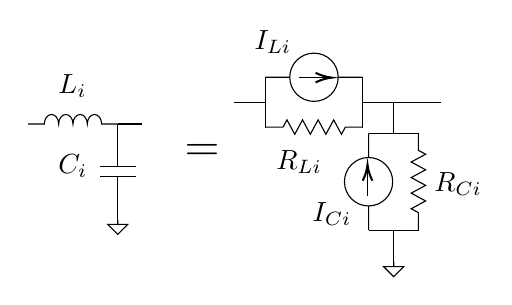
\begin{tikzpicture}[x=0.75pt,y=0.75pt,yscale=-0.7,xscale=0.7]
%uncomment if require: \path (0,196); %set diagram left start at 0, and has height of 196

%Shape: Capacitor [id:dp2252820454824469] 
\draw   (252.6,75.92) -- (252.6,105.46) (264.85,112.02) -- (240.35,112.02) (264.85,105.46) -- (240.35,105.46) (252.6,112.02) -- (252.6,141.57) ;
%Shape: Inductor (Air Core) [id:dp3109211820408735] 
\draw   (191,75.92) -- (202.09,75.92) .. controls (202.09,72.3) and (204.3,69.37) .. (207.02,69.37) .. controls (209.74,69.37) and (211.94,72.3) .. (211.94,75.92) .. controls (211.94,72.3) and (214.15,69.37) .. (216.87,69.37) .. controls (219.59,69.37) and (221.8,72.3) .. (221.8,75.92) .. controls (221.8,72.3) and (224.01,69.37) .. (226.73,69.37) .. controls (229.45,69.37) and (231.66,72.3) .. (231.66,75.92) .. controls (231.66,72.3) and (233.86,69.37) .. (236.58,69.37) .. controls (239.3,69.37) and (241.51,72.3) .. (241.51,75.92) -- (252.6,75.92) ;
%Shape: Ground [id:dp12628201692255892] 
\draw   (259.51,145.02) -- (252.6,151.93) -- (245.69,145.02) -- (259.51,145.02) -- cycle (252.6,141.57) -- (252.6,145.02) ;

%Straight Lines [id:da8406513786670671] 
\draw    (252.6,75.92) -- (269,75.92) ;
%Shape: Output [id:dp010843343795898575] 
\draw   (371,43.74) .. controls (371,34.57) and (378.46,27.14) .. (387.67,27.14) .. controls (396.87,27.14) and (404.33,34.57) .. (404.33,43.74) .. controls (404.33,52.91) and (396.87,60.34) .. (387.67,60.34) .. controls (378.46,60.34) and (371,52.91) .. (371,43.74) -- cycle (354.34,43.74) -- (371,43.74) (420.99,43.74) -- (404.33,43.74) ;
%Shape: Resistor [id:dp014776091197713948] 
\draw   (354.34,78.04) -- (366.4,78.04) -- (369.08,73.08) -- (374.44,83) -- (379.8,73.08) -- (385.16,83) -- (390.52,73.08) -- (395.88,83) -- (401.24,73.08) -- (406.6,83) -- (409.27,78.04) -- (421.33,78.04) ;
%Straight Lines [id:da6632276367303502] 
\draw    (354.34,43.74) -- (354.34,78.33) ;
%Straight Lines [id:da2778675468345144] 
\draw    (420.99,43.74) -- (420.99,78.33) ;
%Straight Lines [id:da4004017749900226] 
\draw    (332.67,61.04) -- (354.34,61.04) ;
%Straight Lines [id:da6297976377401469] 
\draw    (420.99,61.04) -- (442.67,61.04) ;
%Shape: Output [id:dp6982926084202103] 
\draw   (425.25,132.32) .. controls (416.09,132.32) and (408.65,124.86) .. (408.65,115.65) .. controls (408.65,106.45) and (416.09,98.99) .. (425.25,98.99) .. controls (434.42,98.99) and (441.85,106.45) .. (441.85,115.65) .. controls (441.85,124.86) and (434.42,132.32) .. (425.25,132.32) -- cycle (425.25,148.98) -- (425.25,132.32) (425.25,82.33) -- (425.25,98.99) ;
%Shape: Resistor [id:dp6768188450434698] 
\draw   (459.55,148.98) -- (459.55,136.92) -- (454.6,134.24) -- (464.51,128.88) -- (454.6,123.52) -- (464.51,118.16) -- (454.6,112.8) -- (464.51,107.44) -- (454.6,102.08) -- (464.51,96.73) -- (459.55,94.05) -- (459.55,81.99) ;
%Straight Lines [id:da9091970879846805] 
\draw    (425.25,148.98) -- (459.85,148.98) ;
%Straight Lines [id:da8294586622316285] 
\draw    (425.25,82.33) -- (459.85,82.33) ;
%Straight Lines [id:da6048944770810178] 
\draw    (442.55,170.65) -- (442.55,148.98) ;
%Straight Lines [id:da8835570424522978] 
\draw    (442.55,82.33) -- (442.55,60.65) ;

%Straight Lines [id:da19842461223264807] 
\draw    (442.67,61.04) -- (475.33,61.04) ;
%Straight Lines [id:da5573319635988767] 
\draw    (424.53,125.4) -- (424.53,106) ;
\draw [shift={(424.53,104)}, rotate = 90] [color={rgb, 255:red, 0; green, 0; blue, 0 }  ][line width=0.75]    (10.93,-3.29) .. controls (6.95,-1.4) and (3.31,-0.3) .. (0,0) .. controls (3.31,0.3) and (6.95,1.4) .. (10.93,3.29)   ;
%Straight Lines [id:da668789159192102] 
\draw    (377.53,44) -- (397.73,44) ;
\draw [shift={(399.73,44)}, rotate = 180] [color={rgb, 255:red, 0; green, 0; blue, 0 }  ][line width=0.75]    (10.93,-3.29) .. controls (6.95,-1.4) and (3.31,-0.3) .. (0,0) .. controls (3.31,0.3) and (6.95,1.4) .. (10.93,3.29)   ;
%Shape: Ground [id:dp27878598998015525] 
\draw   (449.46,174.11) -- (442.55,181.02) -- (435.64,174.11) -- (449.46,174.11) -- cycle (442.55,170.65) -- (442.55,174.11) ;

% Text Node
\draw (210,95) node [anchor=north west][inner sep=0.75pt]    {$C_{i}$};
% Text Node
\draw (210,40) node [anchor=north west][inner sep=0.75pt]    {$L_{i}$};
% Text Node
\draw (297,88.07) node [anchor=north west][inner sep=0.75pt]  [font=\LARGE]  {$=$};
% Text Node
\draw (345,10) node [anchor=north west][inner sep=0.75pt]    {$I_{Li}$};
% Text Node
\draw (360,92.07) node [anchor=north west][inner sep=0.75pt]    {$R_{Li}$};
% Text Node
\draw (385,128.07) node [anchor=north west][inner sep=0.75pt]    {$I_{Ci}$};
% Text Node
\draw (468.67,107.4) node [anchor=north west][inner sep=0.75pt]    {$R_{Ci}$};


\end{tikzpicture}

    \label{fig:nw_tline_chunk}}
  
  \caption{A transmission line model with $N$ discrete chunks. (a) a typical representation of a lossless transmission line that has $N$ inductor and capacitor (LC) lumped elements in series with each other. On the left $V_{in}(t)$ is an input voltage that varies over time with some input resistance $R_{in}$. A readout voltage $V_{out}(t)$ is induced on the right across the output resistor. (b) an equivalent model used for approximating the transmission line using trapezoidal integration that can also account for DC characteristics and hotspot generation more
  efficiently than its LC counterpart.}
  \label{fig:nw_tline}
\end{figure}

An arbitrary nanowire model can be simulated by repeating ``chunks'' of nonlinear inductors and capacitors
as shown in figure \ref{fig:nw_tline_line}. Using the trapezoidal method on the circuit is equivalent 
to converting each element to a current source and resistor in parallel as shown in figure \ref{fig:nw_tline_chunk} \cite{numerical_integration}. The inductor's non-linear inductance can be encoded
into the resistor and current source by approximating the continuous nonlinearity as linear between two 
successive timesteps. We can then write the general matrix for any nanowire device as follows:
\begin{equation*}
    \begin{bmatrix}
     && \vdots & \vdots & \vdots & & & \\
    &\cdots & -R_{L, i-1} & R_{L, i} + R_{C, i} + R_{L, i-1} & R_{L, i} & \cdots\\
    && \vdots & \vdots & \vdots & \ddots
    \end{bmatrix}
    \begin{bmatrix}
    % v_0\\
    \vdots \\ v_j\\ \vdots
    % \\v_{n+1}
    \end{bmatrix}=
    \begin{bmatrix}
    \vdots \\ i_{L, k} - i_{L, k-1} + i_{C, k-1}\\ \vdots
    \end{bmatrix}
\end{equation*}

The solution for this linear equation is produces the node voltages $v_j$ for the nanowire
between each chunk $j+1$. This is solved for each timestep using the previous timestep
as the initial condition.
In figure \ref{fig:nw_tline_line}, $v_0 = V_{in}$, $v_1$ is $v_0$ minus the voltage drop across
the resistor $R_{in}$ and so on until $v_{n+1}=V_{out}$. The currents $i_{L, k}$ and $i_{C, k}$ 
are the currents going through each inductor $L_k$ and capacitor $C_k$ at a given timestep.

The trapezoidal rule for the inductor above sets the resistor in the companion model shown in figure
\ref{fig:nw_tline_chunk} to $R_{L, i}(t) = \frac{2L}{h}$ for a timestep size of $h$ and unit inductance
$L$. The current source's value would correspond to $i_{L, i}(t) = \frac{h}{2L}v_n(t-\Delta t)+i_{L, i}(t-\Delta t)$ \cite{numerical_integration}. This forms a complete basis for calculating any circuit
parameter and evolving the circuit. 

We can modify this model to account for the nonlinearity by only editing the inductor.
The inductance can be overloaded by changing $L$ to $L(i)$ to account for the continuous 
nonlinearity in inductance. We can also change the inductor's companion resistor value $R_{L, i}$
to account for the hotspot formed when a nanowire switches over the boolean state nonlinearity.
Note that this formulation has implications on any power calculations (for example
when thermally coupling layers) as the current is across both a resistor for the hotspot
and one for the inductor.

\subsection{Kernel}

Our large matrix is sparse and bidiagonal, allowing us to compress the node computations required
to more efficiently simulate the nanowire. Each node on the nanowire is dependent only on the states
of the two adjacent chunks in the previous timestep. This allows us to utilize in-place
loop vectorization on a view of a large state vector with static kernels.

The state vector for the nanowire system is defined as $u = [\; \vec v\; \vec i\; \vec s \;]^T$,
where $\vec v$ and $\vec i$ are the voltages and currents of length $n+1$ and $2n$ for $n$ chunks
respectively. Vector $\vec s$ tracks other system variables such as thermal state (temperature),
hotspot velocity,
normal-superconducting state, resistance, etc. We choose to implement the simulator such that $\vec s = \emptyset$
by default. The hotspot parameters are tracked using a separate precomputed $\vec R$ that is reused for
cases with efficient computation.

We can perform separate repeated computations along 3 different dimensions of $u$, namely, we can
compute $\vec i(t+\Delta)$ based on $u(t)$, then compute $v(t+\Delta)$ from that, followed by
updating any state variables in $\vec s$. This repetition can be optimized and can be exploited using
the concept of views in Julia. A view is a data structure that acts as a matrix or vector where the
underlying values are references to an original matrix or vector. In this example, we can perform
operations on the $n+1$ dimensional vector $\vec v$ efficiently without extracting or copying it from 
the original state variable $\vec u$. 

We can employ \cf{LoopVectorization.jl} to vectorize \cf{for} loops or broadcast operations
to improve runtime performance \cite{julia_loop_vectorization}. 
Loop vectorization
works well in cases where the operations are linear and local. For
example, we can compute $d\vec u$ from $\vec u$ using loop vectorization by formulating
it as \cf{du[i]= CL[i] $*$ (du[i] + R[i] u[i])}. Threads are no longer ordered
and as such, the operations have to be disjoint (user cannot rely on a specific order of
instructions) hence enforcing linearity and locality on vector operations.

kernel - a kernel is a local operation etc. What is the kernel we r using.
% You can think of a Kernel as a function that takes a neighbourhood Window view on the underlying data as an argument. The kernel function aggregates the values within the neighbourhood and outputs a new value. The well-known function map(k, a) applied to the kernel k and a data array a then applies the kernel as a filter.

turbo

views

We can use non-allocating kernel operations using \cf{StaticKernels.jl} to define efficient
quick compiling small kernels \cite{StaticKernels}. 
The defined static kernel speeds up the computation by eliminating
runtime checks, non-allocating operations, introducing boundary conditions efficiently and 
by the automatic vectorization of kernel loops for inlined kernel functions. Given the kernel
we defined for a nanowire device, we can see that the locality of a bidiagonal matrix is an ideal
candidate for using static kernels. We use static kernels on views of $d\vec u$ to generate
new $d\vec v$ and $d\vec i$ values for a given timestep. The kernels we define are local differences
with $k_f$ and $k_b$ being the forward and backwards differences of the vectors, namely $k_f(w)=w[1]-w[0]$
and $k_b(w)=w[0]-w[-1]$. Kernels project a vector to one dimension lower, as a result, we extend the
vectors $d\vec v$ and $d\vec i$ by $V_{in}$ and $\frac{v_n+V_{out}}{R_{out}}$. We then apply 
the static kernel $k_f$ onto $[\vec i, V_{in}]^T$ to get $d\vec v'$ and 
$k_b$ onto $[\vec v, \frac{v_n+V_{out}}{R_{out}}]^T$ to get $d\vec i'$. We can then compute the change
in state vector $d\vec u$ using the loop vectorized expression: \cf{du[i]= CL[i] $*$ (du[i] + R[i] u[i])}.

Inline kernel

\subsection{Modeling the Hotspot}

The simulator models the hotspot using two methods, a pre-computed hotspot evolution
model and using the phenomenological hotspot model used in the SPICE model \cite{karl_spice, phen_model}. 

The pre-computed model consists of a generalized fit for the solution of the hotspot evolution
obtained by simulating the hotspot resistance and scaling its time and amplitude as a function
of the bias current $i$ and the critical current $i_c$. This allows for much faster simulation as you have
less equations coupled, as well as, allowing for better parallelization. In this case, the
hotspot resistance is a linear state evolution as opposed to a coupled nonlinear process. We use
this by caching the hotspot resistance as a vector encoding resistance over discrete timestamps
$\vec R$, where $R_1=0$ and $R_{j} = \max(\vec R)$ for some time $j$. By scaling $j$ and $\max R$ using
a matrix $M_R(i, i_c)$, we can efficiently include the hotspot in the kernel by adding 
$M_R(i, i_c) R_k$. $R_k=R_0$ when the wire is non-switched, and the moment the wire switches,
the state $k$ begins to increment along the dimension of $\vec R$. This formulation can allow
us to not only use it in efficient kernels, but also allows us to cache the value of $\vec R$ 
into a GPUs shared or texture memory to be efficiently reused across the simulation.

\section{ODE Problems and Callbacks}

We use \cf{DifferentialEquations.jl} to repeatedly execute our time-domain kernel evolving our
system in small time steps of variable width $\Delta t$. The \cf{DifferentialEquations.jl} backend
handles timestepping, we force some fixed evaluation times regardless of the variable timestep
method used by \cf{DifferentialEquations.jl}. The \cf{DifferentialEquations.jl} solvers span
benchmark as some of the fastest implementations of some methods as well as being optimized
for high-precision and high-performance compute applications \cite{differentialequationsjl, ODESolver-diffeq}.
The package also supports built-in interpolation, stochastic differential equations, sparsity and 
stiffness detection  as well as arbitrary precision, allowing us to simulate arbitrary dynamics. 
This is important for coupling different types of differential equations to our model to simulate
any arbitrary system on top of a 2-terminal nanowire.

The implemented solver also makes use of discrete and continuous callbacks, periodic checks on conditions
that can be used to modify the behavior of the underlying differential equations. For example, a photon-incidence
event can trigger a discrete callback, making a nanowire element switch into the resistive state at some position.
Additional evaluation times are usually given with a discrete callback to ensure that the problem is evaluated
during the evolution of the callback - in this case, the photon-incidence time would be an additional evaluation
time.
A continuous callback on the other hand involves a time-continuous function where the zero crossings modify
the differential equation behavior. For example, a continuous callback over the value $\Gamma_c(t) = i(x, t)-i_c(x, t)$ 
can track whether a nanowire should be in the superconducting or resistive state. If the nanowire exceeds
the switching current for a time $t' < \Delta t$, a discrete callback on the nanowire simulation will 
likely remain in the superconducting state. However, since the function $\Gamma_c(t)$ is continuous, we
know that a change in sign of $\Gamma_c(t)$ corresponds to a zero-crossing and as such, the wire is much more
likely to accurately switch.

In contrast with the SPICE nanowire model, the switching behaviour on the state non-linearity is much better
defined. We demonstrated in section \ref{stability} that the instability of the nanowire model is strongly
influenced by the harsh state non-linearity. The use of a continuous callback for this nonlinearity makes it
such that the process of entering the resistive state is a linear process. This in effect decreases the coupling
between the timestepping algorithm and the state nonlinearity, allowing for more stable simulations. In the 
picture of projections shown in figure \ref{fig:statespaceevolution}, we filter out cases where we evolve
past the state nonlinearity, project to a state earlier in the state space and then evolve past the nonlinearity
again. This leads to much fewer erroneous switching events.

We can further optimize kernel applications on larger simulations by moving parts of the solver to the GPU. 
This can be done using \cf{CUDA.jl} and is handled by the \cf{DiffEqGPU.jl} backend \cite{CUDAjl, diffeqgpu}. 
We have two ways of compiling GPU kernels: (1) writing a custom GPU kernel optimized for GPU operations and 
(2) rewriting our Julia function so that the \cf{CUDA.jl} package can convert it to an efficient GPU
kernel. The first option is tedious but can provide a lot of optimization for specific problems.
Since our kernel is small and acts locally, this would involve developing a kernel similar to that of 
\cf{prefix-sum} \cite{prefixsumcuda, juliacon_gpu}. The second method offers similar speed-ups with typical 
optimizations such as using views, writing non-allocating code, relying on broadcast operations, etc. 
\cite{juliacon_gpu}. We chose to implement the second method, as it is more easily extendable
if a new type of local coupling is introduced to the nanowire - for example, including thermal effects 
would make a rewritten kernel obsolete.

\subsection{Solvers}

The \cf{DifferentialEquations.jl} package comes with many built-in solvers, all optimized for different
applications \cite{ODESolver-diffeq}. When using above formulations of nanowire nonlinearities using
callbacks, the nanowire simulation is less stiff, allowing us to use non-stiff methods such as \cf{Tsit5}.
\cf{Tsit5} is a modified coefficient tableau for Runge–Kutta 4(5) method developed by Tsitouras
that outperforms other known pairs for medium precision problems \cite{tsit5}. From the multiple methods 
evaluated, \cf{Tsit5} should be used for problems where pulses sent are relatively large and where pulse
reshaping is not important due to \cf{Tsit5}'s lower relative accuracy. It is the fastest of the methods
listed in this section.

When optimizing for higher accuracy, a method like \cf{Vern7} for \cf{Float64} precision (between $10^{-8}\text{ and }10^{-12}$). \cf{Vern9} can be used for bigger tolerances using Julia's 
\cf{BigFloat} type, however, this is not very useful for currently used models of nanowires that
don't require precision below $10^{-12}$. \cf{Vern7} [\cf{Vern9}] is Verner's ``Most Efficient'' 7(6) [9(8)] Runge-Kutta 
method equipped with a lazy 7th [9th] order interpolant \cite{vern}. These two methods can be used in
cases where the simulation is non-stiff but effects like pulse-reshaping and the continuous nonlinearity
exhibited by the inductors matter. These methods are more robust than the equivalent higher order 
Adams-Bashforth methods to discontinuities (as well as are more efficient than the extrapolation
required by Adams-Bashforth methods), which are important for state nonlinearities \cite{ODESolver-diffeq}.

When the problem being simulated is stiff due to coupling with another differential equation, we can
use \cf{Rodas5P} (5th order A-stable stiffly stable Rosenbrock method with a stiff-aware 4th order interpolant)
for medium tolerances \cite{ODESolver-diffeq}. \cf{Rosenbrock23} can also be used for lower accuracy.

\cf{DifferentialEquations.jl} supports composite integration algorithms, with the ability to switch
solvers based on the stiffness. By specifiying a non-stiff and stiff tolerance, we can make a solver switch
between using \cf{Tsit5} (or \cf{Vern7}) when the problem is non-stiff and \cf{Rodas5} when the
solver detects stiffness. The \cf{AutoSwitch} algorithm can decide which method to use from a tuple 
for the next step based on a specified tolerance. The composite algorithms \cf{AutoVern7} and \cf{AutoTsit5} 
are pre-defined and weighted allowing for optimal automatic switching between the a nonstiff and a stiff solver
based on the accuracy required.

Automatic time stepping in \cf{DifferentialEquations.jl} is decoupled from the choice of algorithm.
We use the default Proportional-Integral (PI) controller supplied with \cf{DifferentialEquations.jl}.
This modifies the timestep using a PI controller on the amount of error over time experienced by the
solver \cite{timestepping_alg_PI}. 
This is similar to SPICE implementations, in that the scaled error at a certain timestep is used to either
accept or reject a timestep, then used to calculate the next timestep size if it was rejected.

We might care about the evolution of the entire state vector $\vec u$ and as a result, efficiently
tracking the state vector is important. While all our operations are non-allocating, we can pre-define
timestamps to export the state vector's values at. This allows us to pre-allocate while computing
the evolution in-place unlike in SPICE. The intermediate steps use the interpolation feature provided
in the solvers, allowing us to compute values at well-converging timestamps without computing for the
exact value. This allows us to trade-off the overhead of storing intermediate timesteps while evolving
the state vector.

% \section{Time Domain Reflectometry Example}

\section{Harmonic Balance} \label{julia-sim-hb}

An efficient method used for simulating nonlinear electronics in the frequency domain is harmonic balance
and is the preferred frequency domain simulation implementation in WRspice and Xyce \cite{wrspice, hb-book, xyce_reference}. \cf{JosephsonCircuits.jl} is a Julia implementation that was designed to simulate 
Josephson Traveling Wave Parametric Amplifiers (JTWPAs) in the frequency domain \cite{josephsoncircsjl}. 
It can symbolically produced the nonlinear scattering parameters of long chains of nonlinear devices
that are time decoupled, i.e. if the nonlinearity is a continuous function of current through a device.
This can be an efficient way to produce the frequency response of a nanowire for certain types of inputs
(namely, repeating inputs such as pulse trains) when they are in the superconducting state.

We use the \cf{JosephsonCircuits.jl} solver to produce the nonlinear scattering parameters $S_{xy}(\Tilde i)$
for a device where $x, y\in \{1, 2\}$ and $\Tilde i$ is the ratio of the current flowing through the nanowire
and the switching current. However, we can't use this method to study the state nonlinearity, and as such,
we have to restrict its usage for the continuous state. The output of the simulation is used to assist
the time-domain simulation of long chains by producing a 1-element response oracle, similar to the S-parameter
models generated by \cf{spice-daemon} in section \ref{sparammodels}. 

Given a chain of $N$ uniform nanowire elements in series, we can compute the S-parameter response for a chain 
of length $N/k$ and require $O(k)$ computations to find the response of the device. When the device switches to
the resistive state, instead of simulating the entire $N$ chunks in the time domain, we can now simulate
$k-1$ chunks in the time domain and $N/k+O(k)$ elements in the time domain. This allows us to mix frequency
and time domain models efficiently for nanowire devices that exhibit state nonlinearities. 

Similar to the disclaimer mentioned in section \ref{sparammodels}, care should be taken when mixing frequency and time
domain models as frequency-time domain mixing can cause simulation issues \cite{td-fd-mixing}. This should be
generally avoided as it is now when designing devices that require non-pulse train inputs (even when using 
windowing functions), when used for pulse-reshaping analysis and when we particularly care about the switching
nonlinearity. This method also removes the ability to study nonlinearity transitions using continuous callbacks,
as such it could be detrimental for the performance (and accuracy) of smaller network devices.

\subsection{Device Symmetries}

\begin{figure}
    \centering
    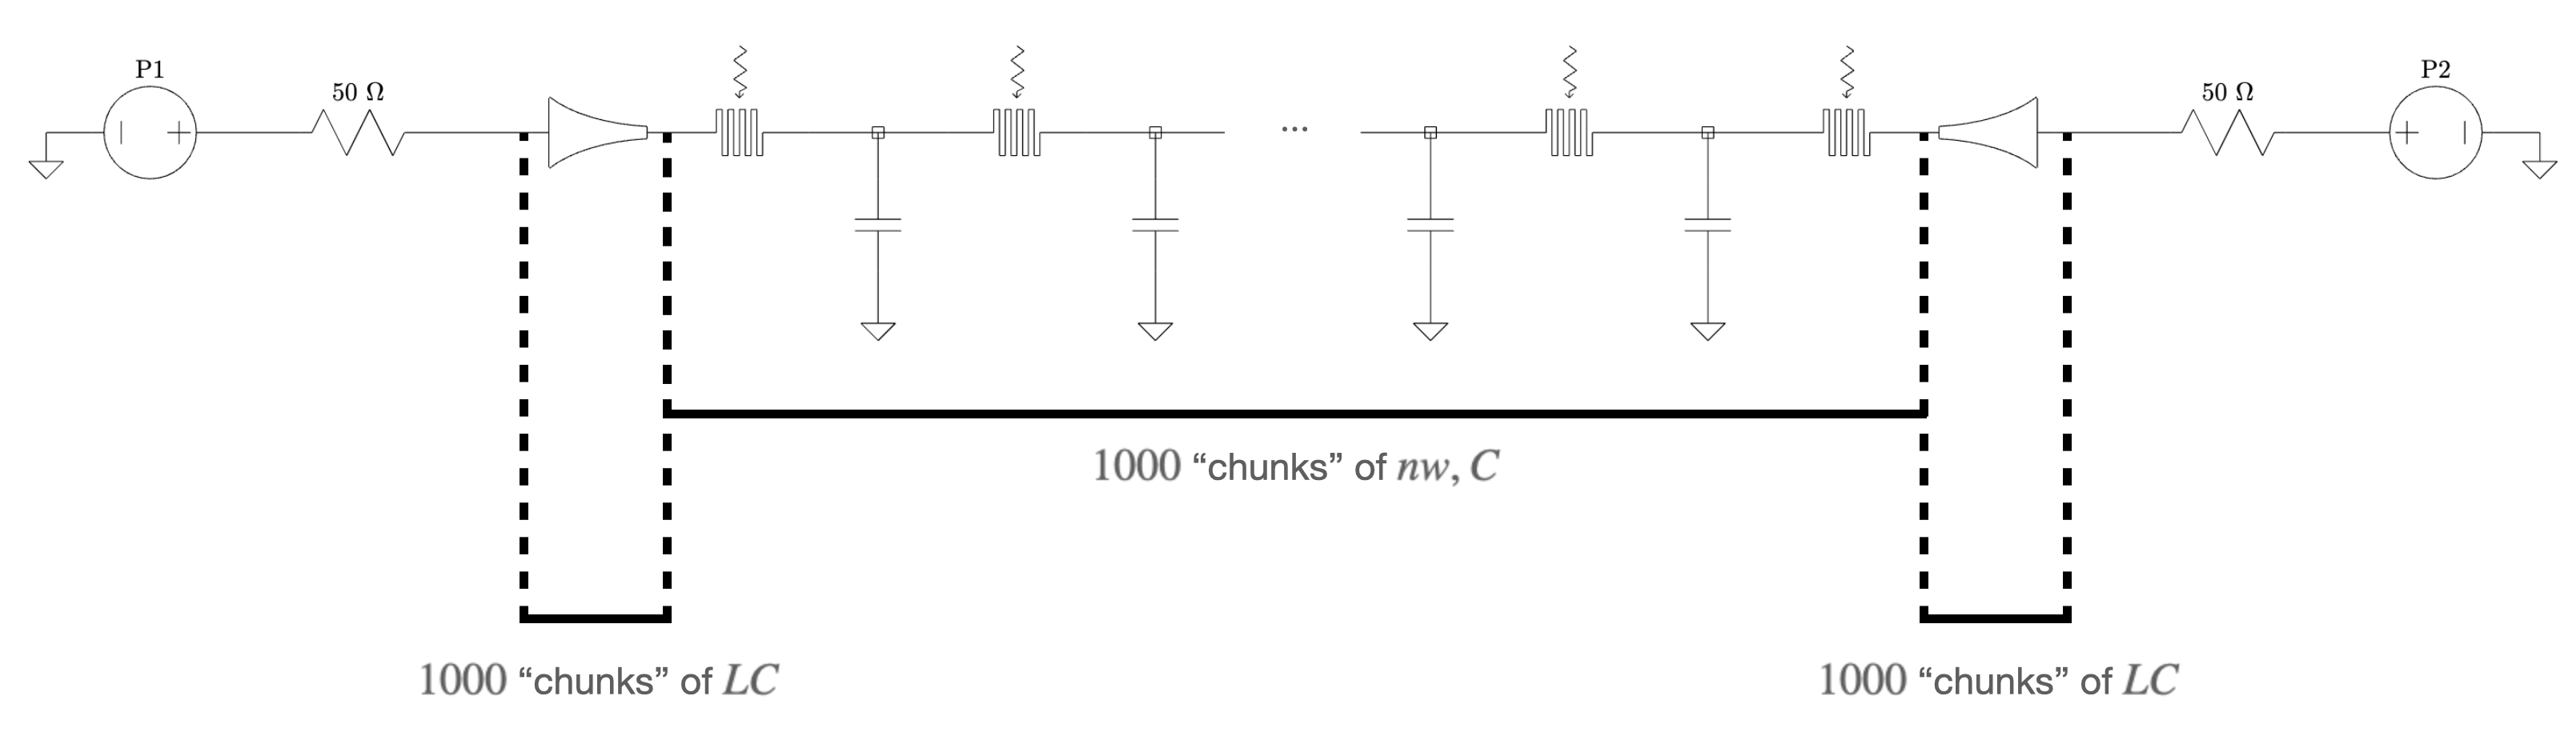
\includegraphics[width=\textwidth]{figs/juliasimsymmetry.png}
    \caption{A typical device layout showcasing multiple device symmetry. The tapers are identical in
    shape and are always superconducting, therefore an efficient oracle can be made for one and reused 
    for the other. The nanowire meander itself is uniform, an oracle for lumps of repeated elements can 
    be used when the wire is superconducting, while the near critical current elements can be simulated
    normally.}
    \label{fig:juliasimsymmetry}
\end{figure}

One particular geometry we care about is simulating a nanowire sandwiched between two impedance-matching tapers.
The tapers usually consist of the same order of number of elements as the nanowire between them. The tapers
tend to be in the superconducting state the majority of the time. Given a promise of them being superconducting
the entire time, we can use the harmonic balance method to generate the taper response. This generates one oracle
to simulate the behaviour of two tapers that were originally on the order of the wire, cutting simulation time by
approximately a third.

\section{Coupling Differential Equations}

Given the use of \cf{DifferentialEquations.jl}, we can have arbitrary systems with arbitrary dynamics
coupled to our nanowire. This can be done by coupling to the state vector $\vec u$ via nodes and/or
by increasing the dimensionality of $\vec u$. For example, we could model thermal transport between
devices on a separate layer, electrically couple devices and differential
equations that govern quantum aspects of a device for qubit applications.

Other than providing the ease of decoupling the actual nanowire solver from arbitrarily complicated
dynamics, this method also allows the \cf{DifferentialEquations.jl} to better utilize the automatic solver
switching algorithm. For a differential equation that is not always active, for example, no heat being generated for the thermal example or no fast pulses travelling in the electrical coupling example,
the dynamics are non-stiff, and the solver can simulate the nanowire using a faster method such as
\cf{Tsit5}. However, when the dynamics evolve to be more complicated, such the hotspot heating a nanowire
above it and nonlinearly changing the pulse shape as a function of time and current through the nanowire,
the solver can switch to a slower stiff solver such as \cf{Rosenbrock23} for the duration of the stiffness.

\subsubsection{Time-to-Digital Converter}

An example simulation includes simulating the heater-tron (hTron) to build a Time-to-Digital Converter
(TDC). We can write out the explicit differential equation for the hotspot using the phenomenological
hotspot model to evolve the evolution of the resistance as a function of the system state $\vec u$. 
Using the power law on the hotspot, we can deduce the amount of thermal energy being dissipated
by the hotspot. We can then model the heat dissipation through the stack and loss to the substrate
using a differential equation governing the electron-phonon interactions between the layers of the stack.
Using this picture, we can extract how much each layer heats up, and see how that heating up affects
a separate nanowire, allowing it to switch. We can construct a TDC by laying out $N$ parallel 
lines biased by a current perpendicular to one clock line. 
The clock line has a pulse train at a frequency $f$ and a duty cycle 
$<<\frac{1}{f}$ travelling down it from port 1. An input pulse at port 2 will intersect the pulse train 
at a position, forming a hotspot and locally heating up the wire. The thermal coupling to the second
layer switches the top device, causing a readout pulse on one of the $N$ lines. 

\subsubsection{SNSPI coupling}

Modeling the electrostatic coupling between lines on a microstrip architecture can be done
to optimize device shape for optimal pulse readout. When designing a microstrip SNSPI, the
conducting/superconducting meander is coupled to the ground plane vertically. Unlike in a 
Co-Planar Waveguide (CPW) geometry, the meander is not surrounded by ground on the same plane, 
and as a result the waveguide experiences much more capacitive coupling. Building a 
microstrip-based SNSPI with a densely packed meander causes pulses to reshape and
arrive earlier at the readout ports as illustrated in figure \ref{fig:snspi_coupled}. 
This makes it harder to use the SNSPI in its intended
fashion of timing pulses. As a result, simulating the electrostatic coupling between multiple
lines as a function of the width is useful. We can find the optimal ratio $C_c/C_g$, where $C_c$
is the coupling between different microstrip lines and $C_g$ is the coupling to ground,
for a uniformly spaced line optimizing for the readout pulse distinguish-ability while trying to 
maximize $C_c$ for a given line. In other words, we can find the maximally densely packed 
SNSPI line that still has the least amount of coupling between the lines.

\begin{figure}
    \centering
    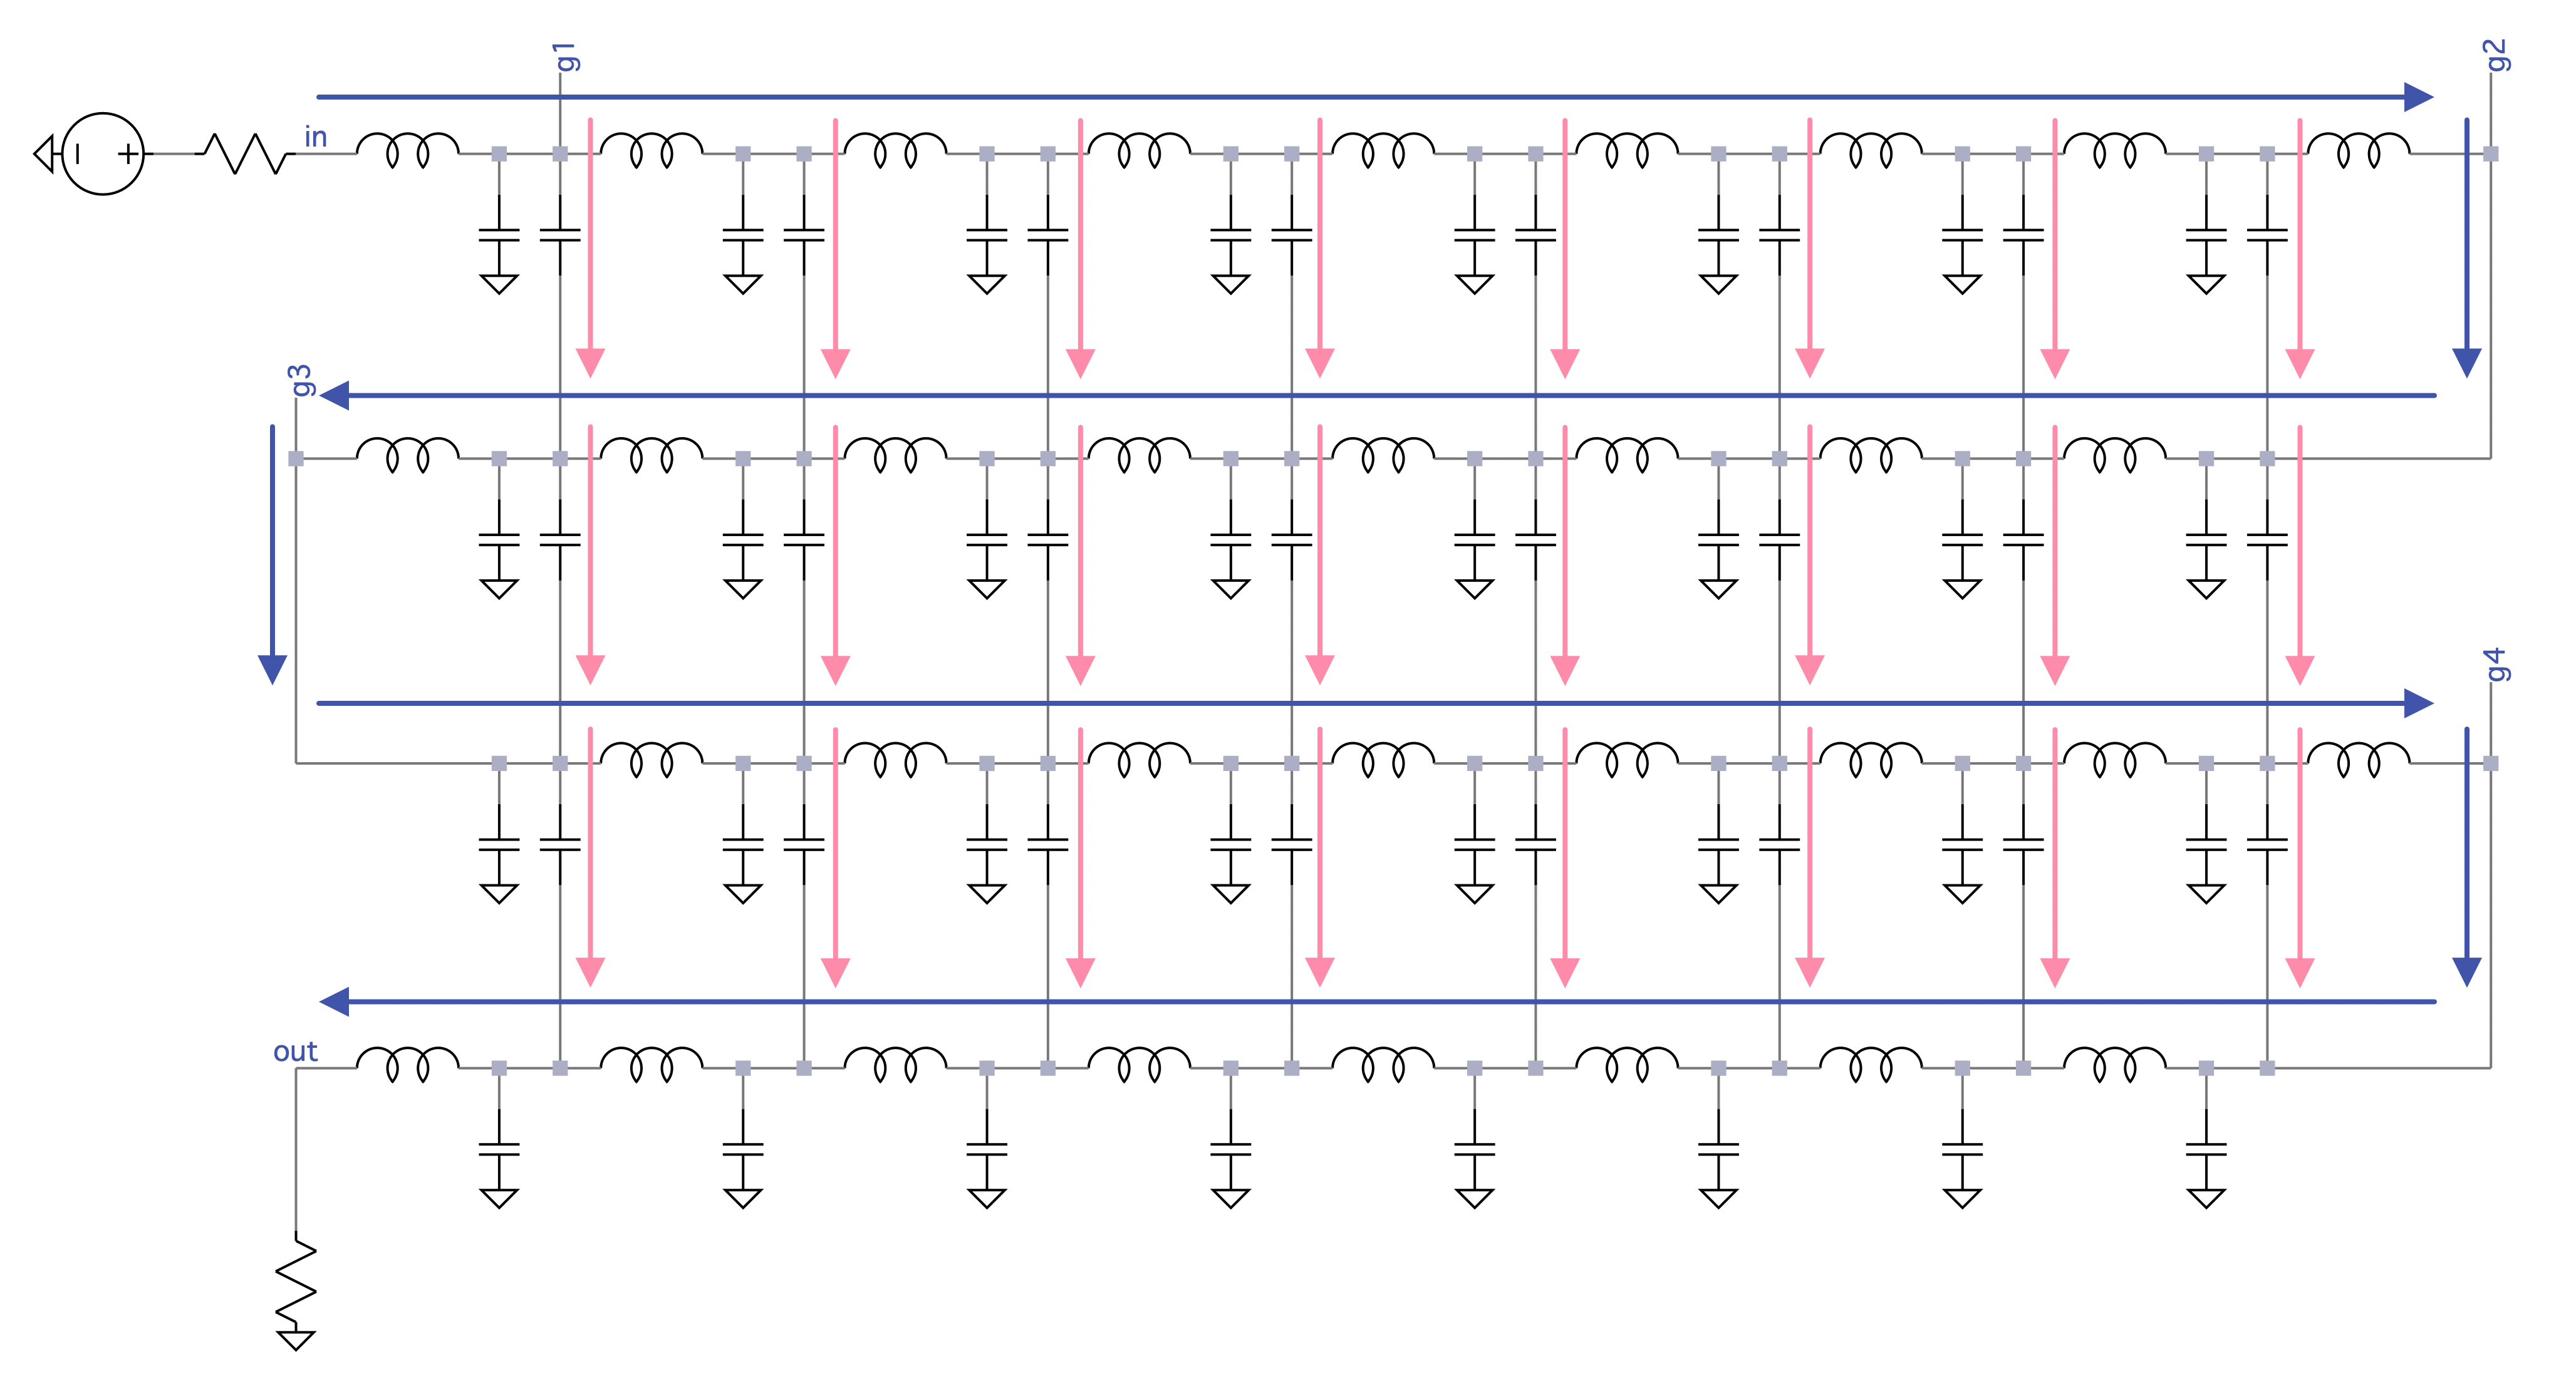
\includegraphics[width=0.8\textwidth]{figs/snspi_coupled.png}
    \caption{Circuit topology for a self-coupled microstrip SNSPI. As the coupling between
    the lines increases, an input signal supposed to travel down the blue path is more 
    likely to couple across and travel along an alternate pink path. The ratio of the coupling to ground $C_g$
    and coupling between adjacent lines $C_c$ controls how much the signal is transmitted along the blue
    versus pink paths.}
    \label{fig:snspi_coupled}
\end{figure}

This topology requires coupling every $2k$ nanowire elements to another $2k$ elements in an alternating 
fashion for an SNSPI meander simulated with $N$ nanowire elements and $N/k$ folds. This forms a square
grid with $k^2$ connections, forming a stiff problem that loses the advantages introduced by the
nanowire optimized simulator for 2-terminal devices. This can be overcome by introducing a separate
differential equation that is coupled to $\vec u$. This coupling works using the equation of a capacitor
between each node $n$ and node $n+k$ and $n-k$. This separate coupling can also be made sparse, such that
it is not computed for nodes with voltages below a certain threshold. As such, the network being simulated
is a 2-terminal device except for when a voltage pulse is being dissipated along the meander.
This preserves the optimizations granted by the 2-port model while being equivalent to the $O(N^2)$
coupled model.

\begin{figure}
    \centering
    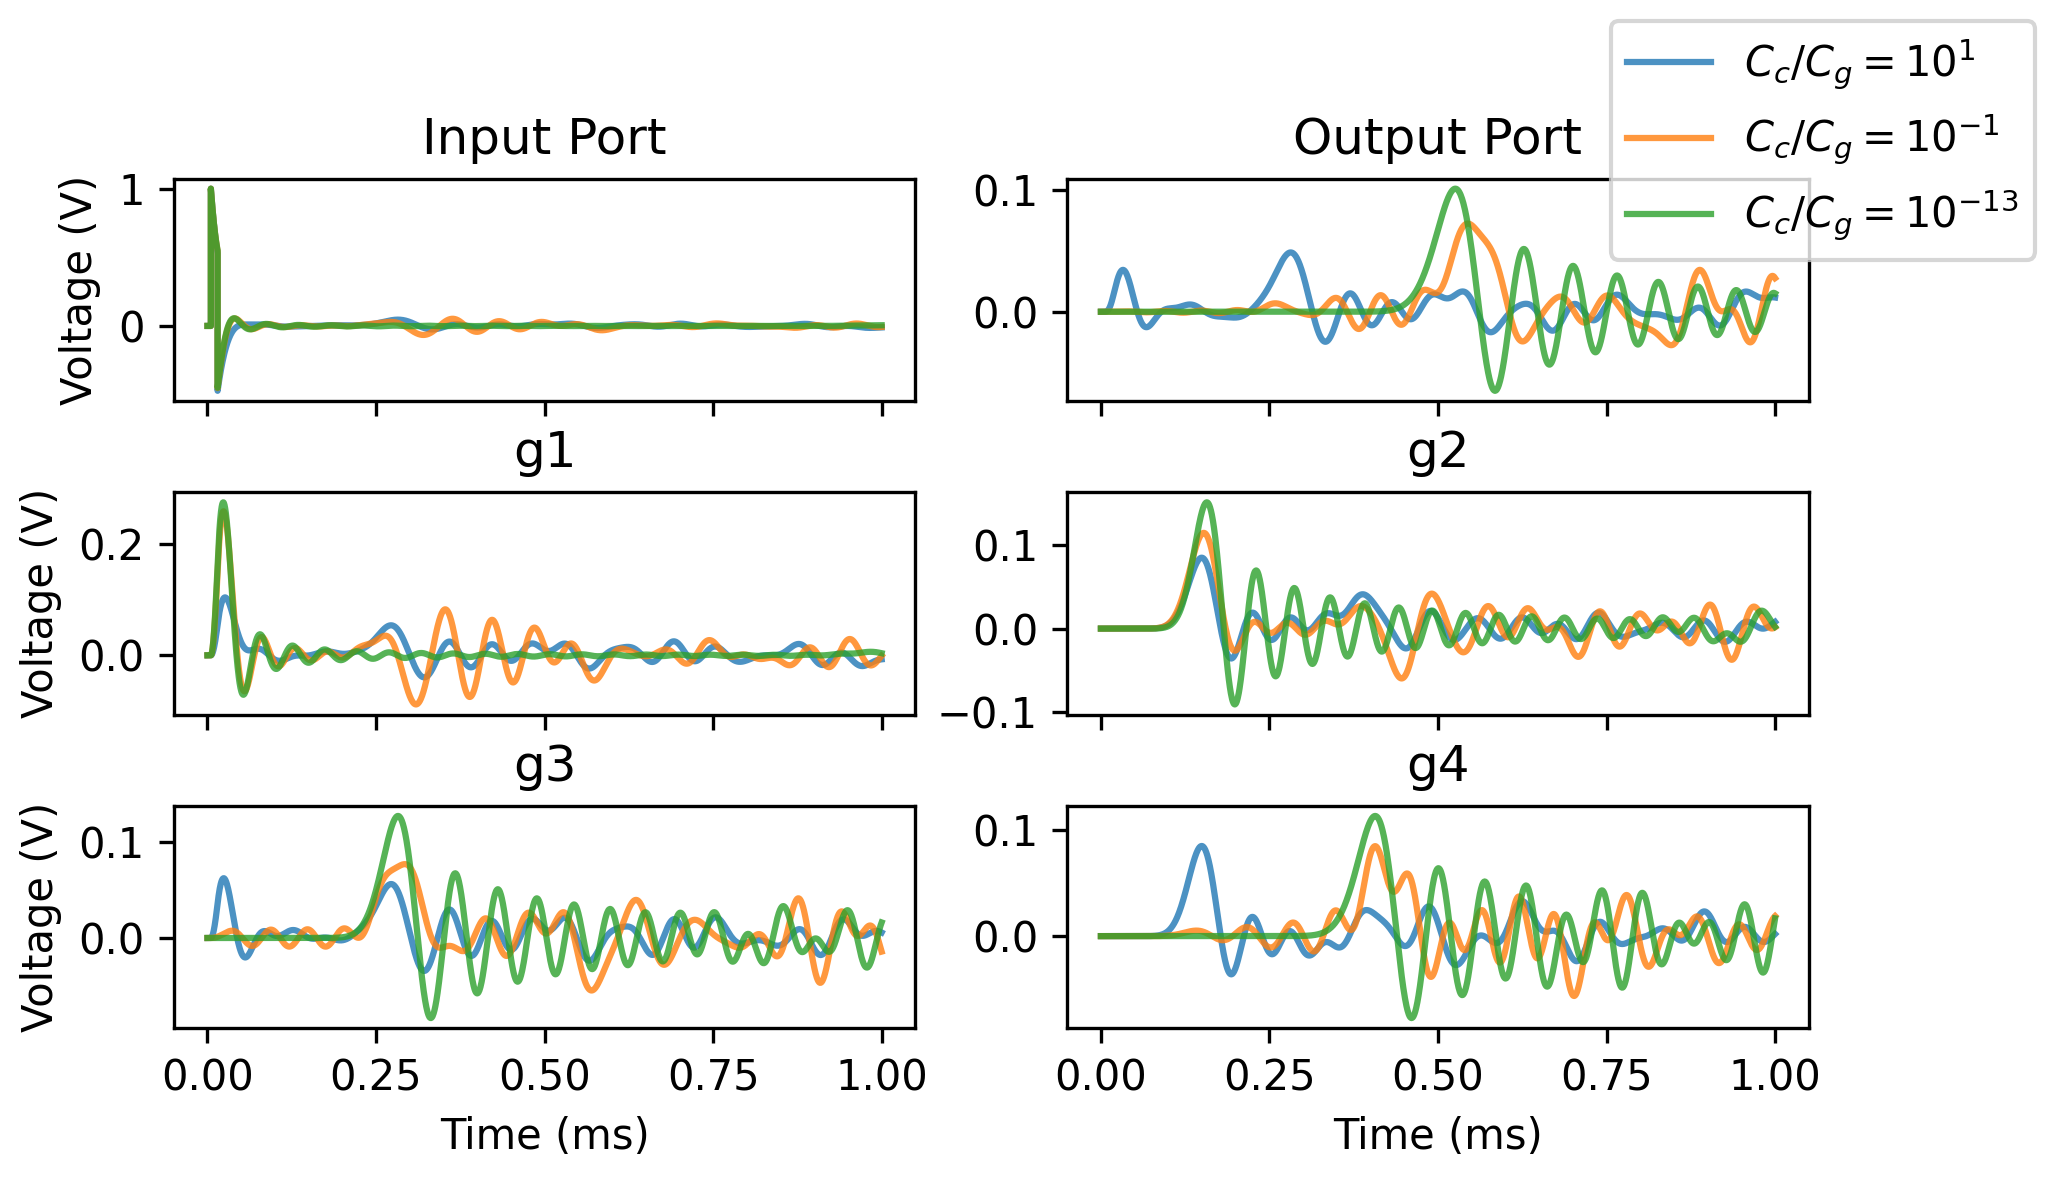
\includegraphics[width=0.8\textwidth]{figs/snspi_coupled_data.png}
    \caption{Simulation results for $C_c/C_g\in \{ 10^1, 10^{-1}, 10^{-13}\}$ showcasing
    the input and output ports, as well as 4 inflection points in the meander.}
    \label{fig:snspi_coupled}
\end{figure}

\section{Automated Taper Optimization}

One of the benefits introduced by a fast solver is the ability to run multiple iterations varying a
single parameter to optimize your design. One particular optimization example is using gradient descent
to improve a design parameter. We can use packages like \cf{Flux.jl} and \cf{Optim.jl} to run standard
machine learning methods on differential equations \cite{fluxjl, optimjl}.

We used \cf{Optim.jl}'s Nelder–Mead method to design an optimized taper in conjunction with the
harmonic balance backend. A linear taper of length $l$ can be fully defined using two 
functions $L(x)$ and $C(x)$ for $x\in[0, l]$.
By computing the scattering parameters for the linear taper, we can perturb $L(x), C(x)$ to
find a more optimal geometry. The Nelder-Mead method is gradient free and as such, involves
repeatedly evaluating multiple small perturbations. As such using it on the entirety of the 
discretization of the taper is too much. We define perturbing $L(x)$ and $C(x)$ as perturbing
two vectors $\vec v_L$ and $\vec v_C$ of a dimension smaller than the discretization size.
For example, we can simulate a taper using $10,000$ nanowire elements and set the dimensions of
the perturbation vectors to $100$ dimensions. We can then interpolate $100,000$ $L(x)$ values 
from $100$ parameters.

Given the condition that impedance-matching tapers should be smooth to decrease reflections,
the abstraction of $\vec v_L$ and $\vec v_C$ preserves smoothness for tiny perturbations.
Starting from a reflection optimized taper, such as a Klopfenstein taper, we can perturb
it to optimize for a specific application \cite{klopfenstein_transmission_1956}.

We define a composite loss function 
$f_{S_{11}} + f_{Z, \text{input}} + f_{\text{illegal}}$ 
that perturbs the inductances and capacitances
of a symbolically generated taper. The first component is an optimization over the taper's
scattering parameters. Given the $S_{11}(\omega)$ parameters of the taper (a complete basis for a
superconducting 2 port device), we construct two sigmoid shaped filters around a design
frequency to separate $\omega$ into two bands ($\omega_\downarrow$ and $\omega_\uparrow$), we
used the design frequency of $2$\si{MHz}. 
Ideally, we want one band to be purely passive, while the other is purely reflective.
Given a stop band suppression of $k_S$ \si{dB}, we have the following loss function:

$$f_{S_{11}} = \sum_{\omega \in \omega_\downarrow} \left ( S_{11}(\omega) \cdot \dfrac{1}{1+\exp {(k_1 (\omega - k_S )) }} \right ) + \sum_{\omega \in \omega_\uparrow} \left ( S_{11}(\omega) \cdot \dfrac{1}{1+\exp {(-k_1 \omega) }} \right ) $$

$f_{Z, \text{input}}$ ensures the input and output ports are impedance matched, i.e.

$$f_{Z, \text{input}} = k_2 \left (  
\left |   Z_{in} - \sqrt{L(0)/C(0)}    \right | +
\left |   Z_{out} - \sqrt{L(l)/C(l)}    \right |
\right)$$

and, $f_{\text{illegal}}$ bounds our inductance and capacitance to be strictly above $0$, i.e.

$$f_{\text{illegal}} = \begin{cases}
        k_3 & \text{if } L(x), C(x) < 0\;\; \forall\; x\in [0, L]\\
        0 & \text{otherwise }
    \end{cases}
$$

with three scaling parameters $k_1, k_2$ and $k_3$, (we used $-20, 10, 100$ respectively). Using
Nelder-Mead on the fitted taper parameters, initial conditions of a Klopfesntein taper with some noise, 
simulated using the harmonic balance backend, we 
generated an optimized taper compared in figure \ref{fig:taper_optim} to a Klopfesntein taper.

\begin{figure}
    \centering
    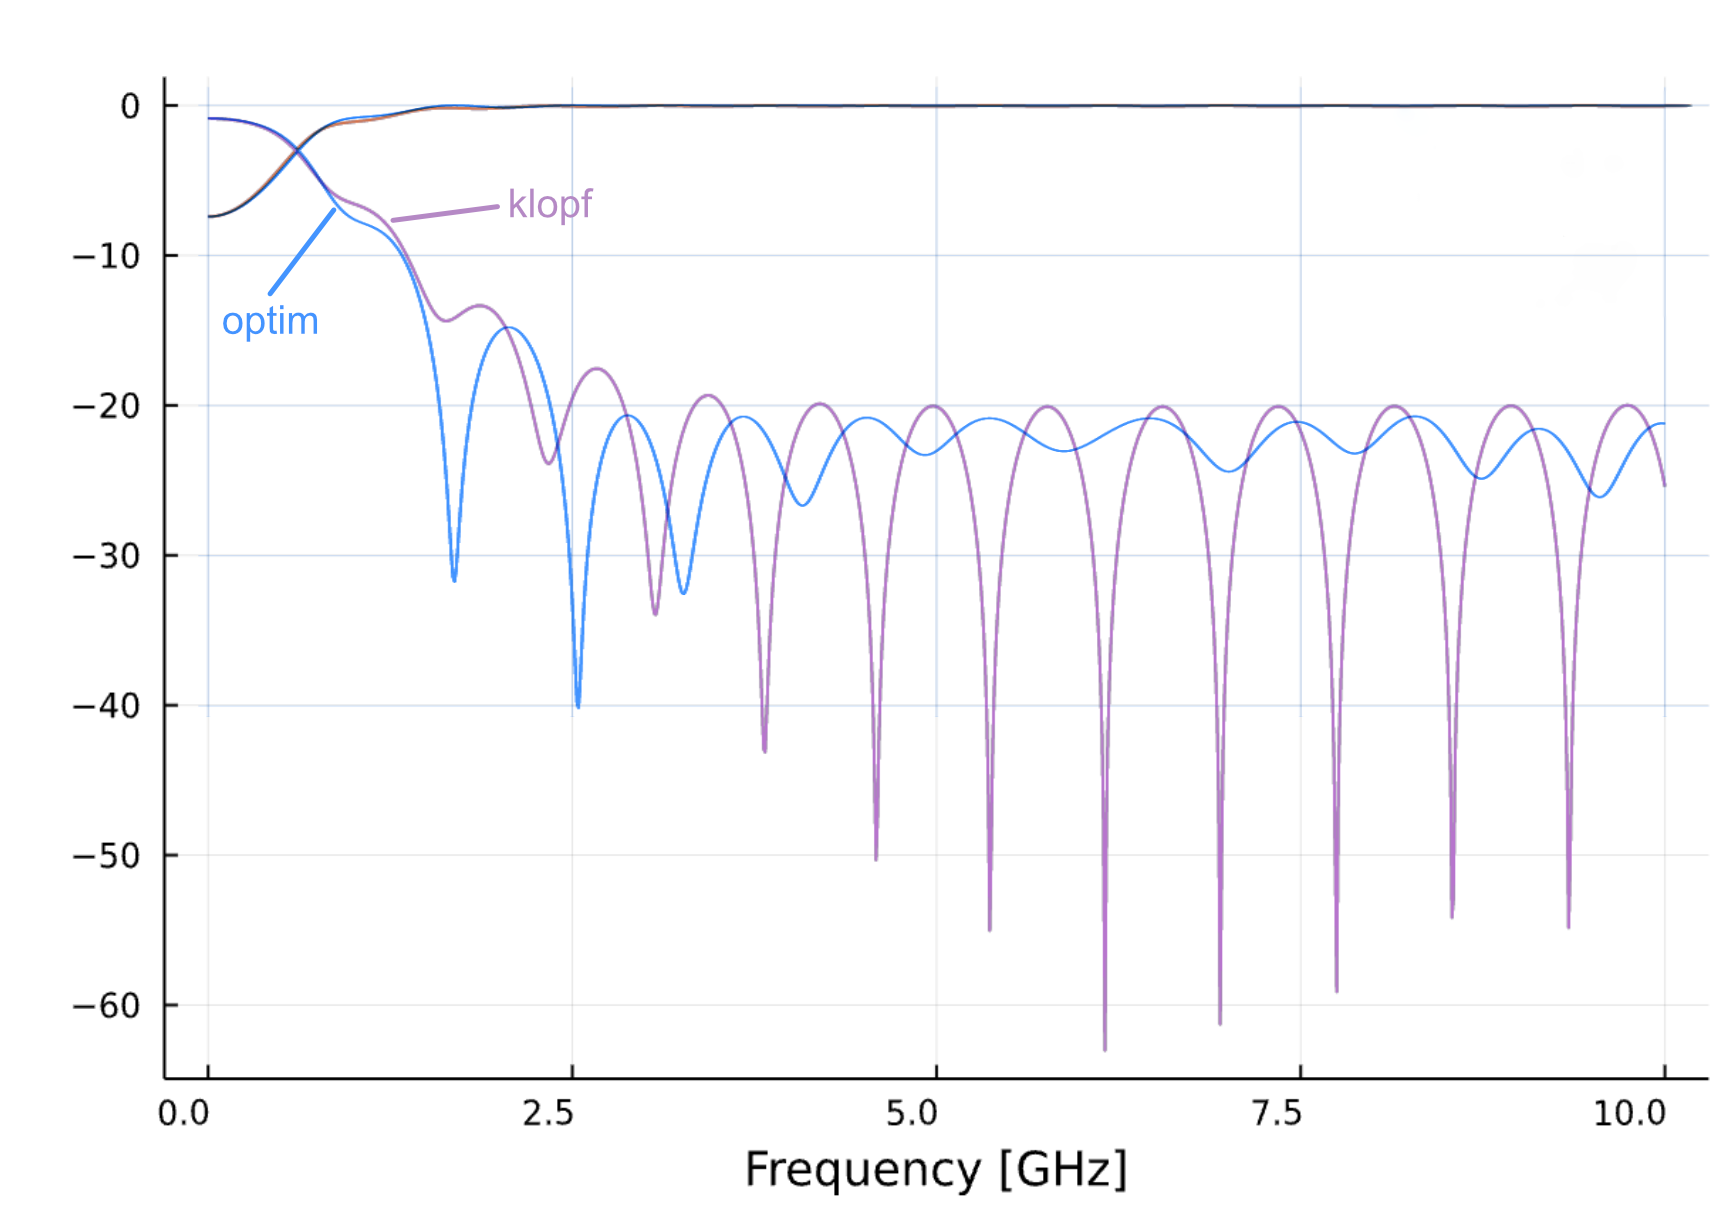
\includegraphics[width=0.6\textwidth]{figs/optim_taper_preliminary_results copy.png}
    \caption{An optimized taper's scattering parameters compared to that of a Klopfenstein taper. The taper
    was optimized using the Julia simulator and \cf{Optim.jl}'s Nelder-Mead method.}
    \label{fig:taper_optim}
\end{figure}

This optimization uses Julia's symbolic capabilities, allowing it to be much more efficient.
By computing a symbolic version of the harmonic balance problem, modifications to circuit
parameters can be recomupted efficiently. This fast recomputation is useful for optimization
methods such as Nelder-Mead since the bulk of the computation is done in the first iteration
and a less substantial computation is used for the optimization parts.

A further optimization to this would rely on building a differentiable simulator.
In its current form, \cf{JosephsonCircuits.jl} computes the harmonic balance
solution using \cf{FFTW.jl} and \cf{KLU.jl}, both of which are wrappers for
non-Julia native programs (the C implementations of
\cf{FFTW} and KLU in \cf{SuiteSparse}) \cite{fftwjl, klujl, 
fftw, klu}. This reliance on non-Julia natives takes away the automatic differentiation
features introduced by Julia. Julia's auto-differentiation allows packages like \cf{Flux.jl}
to take derivatives of functions, and as such, find gradients along a parameter space \cite{fluxjl}. 
These gradients are useful for optimization and allow for faster convergence. Nelder-Mead
is a gradient-free method.